\section{Mixed Cell Volume Radionuclide Model}\label{sec:mixed_cell}

    % WF : glass 

      % alteration

      % temperature limit

    % WF : uox 

      % cladding limit

      % corrosion

A main nuclide transport component model used in this work is a mixed cell 
component module incorporating solubility and sorption effects as well as  
engineered material dissolution.

A graphical representation of the mixed cell model is given in Figures 

\ref{fig:intact} and \ref{fig:dissolved}. 

\begin{figure}[h!]
\begin{minipage}[b]{0.5\linewidth}
  \begin{center}
    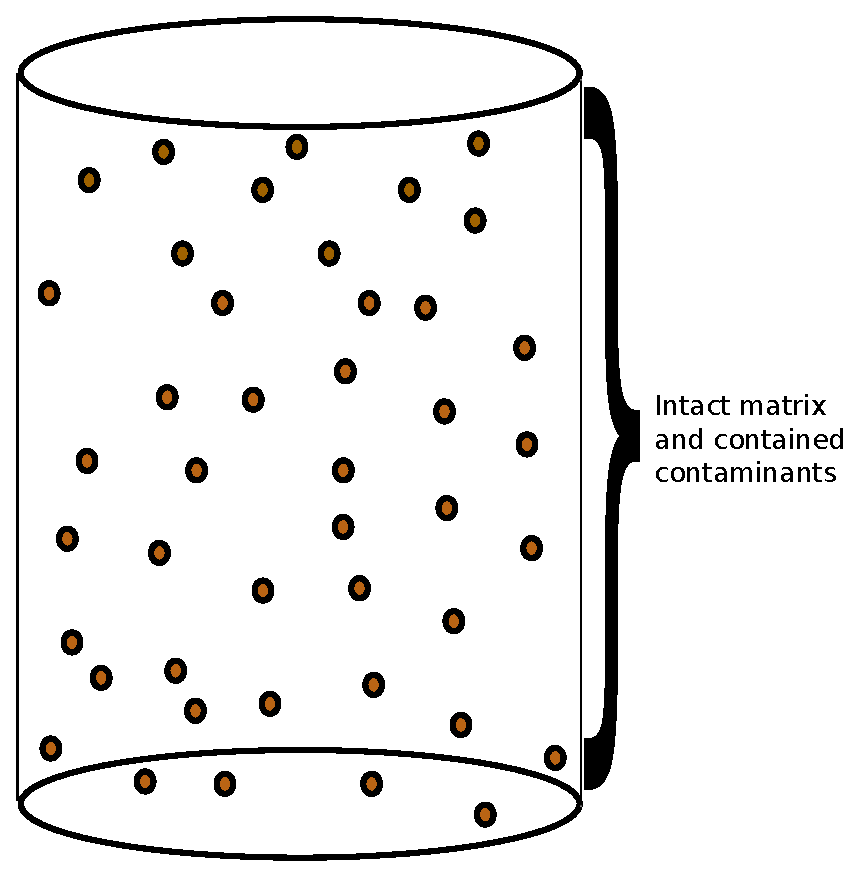
\includegraphics[height=7cm]{./chapters/future/contaminated1.eps}
  \end{center}
  \caption[Intact Mixed Cell Control Volume]{The control volume contains an 
  intact material matrix and contaminants that are unavailable to neighboring 
  subcomponents until dissolution has begun.}
  \label{fig:intact}
\end{minipage}
\hspace{0.5cm}
\begin{minipage}[b]{0.5\linewidth}
  \begin{center}
    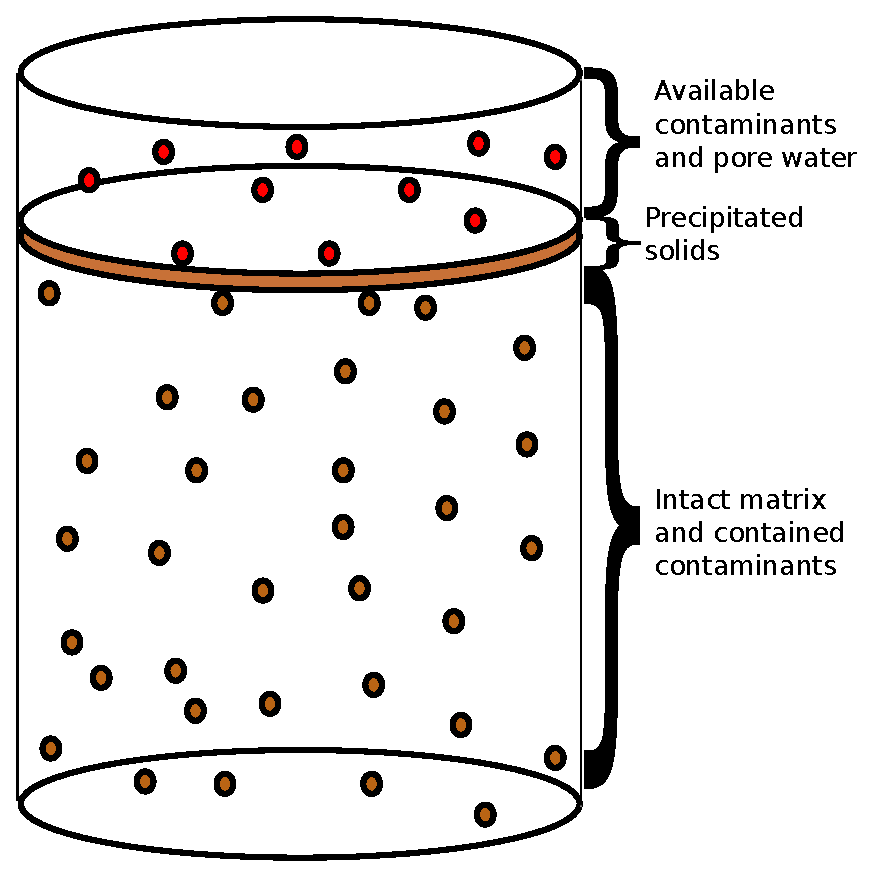
\includegraphics[height=7cm]{./chapters/future/contaminated.eps}
  \end{center}
  \caption[Degrading Mixed Cell Control Volume]{Once dissolution begins, the 
  control volume contains a partially dissolved material matrix, contaminated 
  pore water, and precipitated solids.}
  \label{fig:dissolved}
\end{minipage}
\end{figure}

